% interactcadsample.tex
% v1.03 - April 2017

\documentclass[]{interact}

\usepackage{epstopdf}% To incorporate .eps illustrations using PDFLaTeX, etc.
\usepackage{subfigure}% Support for small, `sub' figures and tables
%\usepackage[nolists,tablesfirst]{endfloat}% To `separate' figures and tables from text if required

\usepackage{natbib}% Citation support using natbib.sty
\bibpunct[, ]{(}{)}{;}{a}{}{,}% Citation support using natbib.sty
\renewcommand\bibfont{\fontsize{10}{12}\selectfont}% Bibliography support using natbib.sty

\theoremstyle{plain}% Theorem-like structures provided by amsthm.sty
\newtheorem{theorem}{Theorem}[section]
\newtheorem{lemma}[theorem]{Lemma}
\newtheorem{corollary}[theorem]{Corollary}
\newtheorem{proposition}[theorem]{Proposition}

\theoremstyle{definition}
\newtheorem{definition}[theorem]{Definition}
\newtheorem{example}[theorem]{Example}

\theoremstyle{remark}
\newtheorem{remark}{Remark}
\newtheorem{notation}{Notation}


% tightlist command for lists without linebreak
\providecommand{\tightlist}{%
  \setlength{\itemsep}{0pt}\setlength{\parskip}{0pt}}



\usepackage{hyperref}
\usepackage[utf8]{inputenc}
\def\tightlist{}


\begin{document}


\articletype{ORIGINAL RESEARCH CHAPTER}

\title{Mortuary assemblage diversity, Gahagan bifaces, and the evolution
of a Caddo burial tradition in the American Southeast}


\author{\name{Robert Z. Selden, Jr.$^{a}$, John E. Dockall$^{b}$, and
David L. Carlson$^{c}$}
\affil{$^{a}$Heritage Research Center and Department of Biology, Stephen
F. Austin State University; Cultural Heritage Department, Jean Monnet
University; $^{b}$Stantec, Inc.; $^{c}$Department of Anthropology, Texas
A\&M University}
}

\thanks{CONTACT Robert Z. Selden,
Jr.. Email: \href{mailto:zselden@sfasu.edu}{\nolinkurl{zselden@sfasu.edu}}, John
E.
Dockall. Email: \href{mailto:johnd@coxmcclain.com}{\nolinkurl{johnd@coxmcclain.com}}, and
David L.
Carlson. Email: \href{mailto:dcarlson@tamu.edu}{\nolinkurl{dcarlson@tamu.edu}}}

\maketitle

\begin{abstract}
Contextual differences in Caddo burials that included Gahagan bifaces
indicate two discrete burial traditions; one where a biface was placed
\emph{atop or alongside an individual} and another where a cache of
Gahagan bifaces was placed \emph{along the northern wall of the burial
feature}. This exploratory study asks whether assemblage diversity and
evenness, for mortuary contexts associated with Gahagan bifaces,
increases through time, and whether Gahagan biface morphology may differ
based on context. A seriation of mortuary contexts paired with an
analysis of mortuary assemblage diversity highlights changes in Caddo
burial assemblages through time, where the earliest contexts express
lower diversity and evenness than later contexts. Results also indicate
that Gahagan biface morphology differs between Caddo burial traditions,
indicating discrete communities of practice related to object placement
and shape preference. These findings provide the basis for a discussion
of the establishment, maintenance, and evolution of a Caddo burial
practice that occurs during the transition from a mobile horticulturist
lifeway to one of emergent---and more sedentary---agriculturalists.
\end{abstract}

\begin{keywords}
American Southeast; Caddo; NAGPRA; archaeoinformatics; network analysis;
assemblage diversity; 3D geometric morphometrics; museum studies;
digital humanities
\end{keywords}

\begin{quote}
Studying the history of paper exposes a number of historical
misconceptions, the most important of which is this technological
fallacy: the idea that technology changes society. It is exactly the
reverse. Society develops technology to address the chages that are
taking place within it \citep[xiv]{RN10878}.
\end{quote}

\hypertarget{introduction}{%
\section{Introduction}\label{introduction}}

The presence of large bifaces as part of lithic assemblages across the
American Southeast originated during the Early to Middle Archaic period,
was associated with several major cultural and technological changes,
and continued into the Woodland and Mississippian periods. Cultural
changes coincided with shifts in residential mobility, and abbreviated
territories. The major characteristics of Middle Archaic organization
that aided in setting the stage for an emphasis on large bifaces
included: (1) decreased scale of land use; (2) increased emphasis on
local raw material sources; (3) an emphasis on expediency; and (4) an
increase in residential mobility (Amick and Carr 1996:53). Across the
American Southeast from the Middle to Late Archaic was an increasing
emphasis on the use of certain nonlocal raw materials, some aspects of
the technology became less expedient with a greater reliance on hafting
and bifaces and increased logistical mobility. Concomitant with a period
of decreased scales of land use, limited areal mobility, and
technological shifts emphasizing larger hafted bifaces and specific raw
materials, social and economic factors fostered the development of
complex and large-scale exchange networks across the region (Jeffries
1996:223). Increasing sedentism across the Archaic period into the
Woodland and Mississippian periods appears to have been connected to
strategies for hunter-gatherer groups to maintain territorial boundaries
and spacing between adjacent groups (Brown 1985:224; Rolingson and
Mainfort, Jr., 2002). Exchange networks and interaction spheres
functioned to maintain and formalize regional boundaries, territories
and intergroup relationships. In such settings, large formal bifaces and
other artifact types became stylistic items of exchange and boundary
markers. Brose (1979:6) noted that such stylistic marker items often
appear among similar ethnic groups occupying the same
cultural-ecological system. The presence of boundaries, formalized by
exchange relationships and codified by stylistic markers (artifacts)
contributed to ecological stability, access to important resources, and
group protection (see Jeffries 1996:227).

Sassaman (2010:99-105) provides an excellent survey of the large bifaces
in the American southeast that were key items of large regional exchange
networks and interaction spheres. Formal hafted bifaces were
characteristic of the entire Archaic period. These items typically
functioned as knives, projectile points, and cores in both hafted and
unhafted forms. Bifaces also functioned and fulfilled major symbolic
roles as exchange items, individual status markers, and as mortuary
items, in addition to their functional roles in subsistence and defense.
Consequently, the procurement of raw materials and manufacture of formal
hafted and unhafted bifaces often exhibited unique characteristics:
exotic and nonlocal raw materials, exaggerations of form, and mass
manufacture by craft specialists in dedicated workshop areas. Those
bifaces that were incorporated into ceremonial contexts were often used
in mortuary functions as grave goods, dedicatory caches for mound
building or mortuary purposes, ceremonially broken or burned. A variety
of formal biface types across the Archaic period functioned in
non-subsistence roles (Sassaman 2010). These included the large Dalton
points in the central Mississippi Valley (Futato 1983; Gramly and Funk
1991; Morse 1997), Benton points and cache blades of the middle
Tennessee River valley and northern Alabama and Mississippi (Johnson and
Brooks 1989), Middle Archaic biface caches of the Midwestern mortuary
complexes in Illinois and Missouri areas (see Hassen and Farnsworth
1987; O'Brien and Wood 1998), Susquehanna biface traditions along the
Eastern Seaboard and Middle Atlantic coast (Dincauze 1968), and Red
Ochre cache blades along the Ohio and Illinois River valleys and
extending into the northeastern United States (see Granger 1978; Pleger
2000). In some areas of the United States, these traditions of large
formal bifaces continued and include such types as Gahagan and Copena
(which are included as part of the topic of this paper and others OUR
REFS HERE). Sassaman (2010:104-105) duly notes that the presence of
bifaces in burials or as nonmortuary offerings or caches is not unique
to the Archaic period. However, the manufacture and caching of very
large bifaces, unusual forms, or large numbers of preforms appears to
have occurred in a limited number of areas for short periods of time. He
also noted that there was a general trend across the Archaic and later
time periods for decreased size of most bifaces but an increase in the
numbers of bifaces included in large caches (Sassaman 2010:105). For
many of these biface traditions, it was common to include smaller and
more worn or utilized examples as components to the cache or mortuary
feature, a trend also observed among Gahagan and Copena biface types.
This dichotomy of bifaces, while not understood, was undoubtedly
significant to the event at hand, and may have indicated that the
spatial separation of the dead from the living was not entirely
clear-cut in society. Gahagan and Copena biface styles and their use in
mortuary and non-mortuary ceremonial or dedicatory cache offerings may
represent part of the terminal end of the large bifaces in the American
Southeast phenomenon that appears to have begun during the Late
Paleoindian-Early Archaic Transition but reaching its culmination during
the Middle to Late Archaic.

Found to occur along the western margin of the American Southeast,
Gahagan bifaces are among the most recognizable and well known
components of Caddo material culture, and were regularly included with
burial offerings during the Formative (CE 800-1000) and Early (CE
1000-1250) Caddo periods
\citep{RN7115,RN8189,RN5746,RN8186,RN8174,RN8176}. Recent efforts to
characterize general trends associated with Gahagan biface morphology
yielded support for a \texttt{spatial\ boundary} that divides the
northern and southern Caddo behavioral regions based upon morphological
differences that occur in Caddo bottles, Gahagan bifaces, and Perdiz
arrow points (\textbf{\texttt{Chapter\ X,\ Figure\ 1c}})
\citep{RN7925,RN8071,RN8361,RN8967,RN11064,RN8154}. A second
\texttt{shape\ boundary} has also been posited based upon differences in
Gahagan biface morphology between the Caddo and central Texas regions
\citep{RN8318}.

\begin{figure}

{\centering 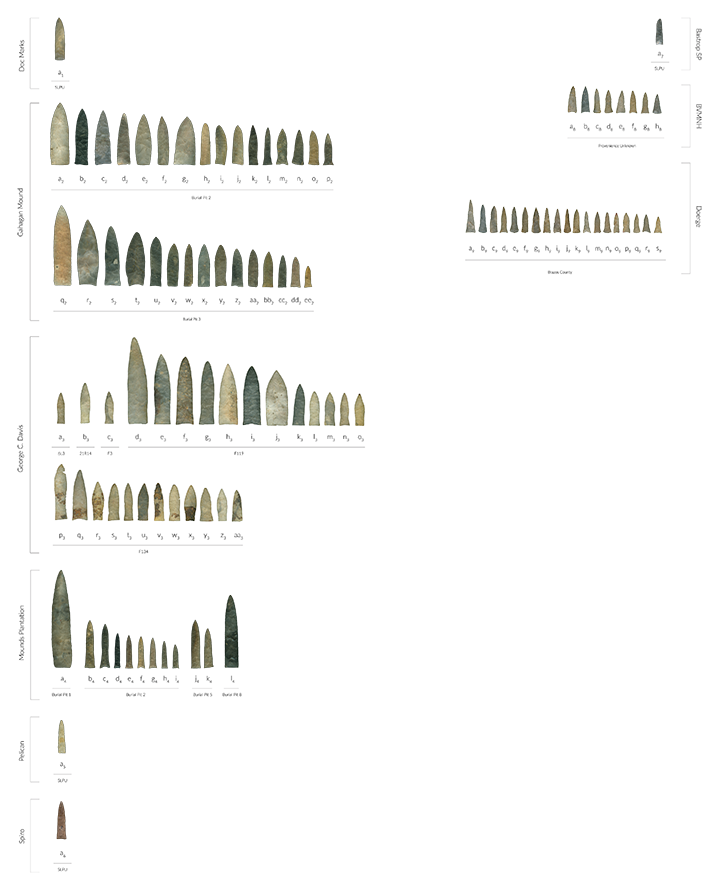
\includegraphics[width=0.8\linewidth]{img/fig02} 

}

\caption{Gahagan bifaces from the northern and southern Caddo behavioral regions. Bifaces recovered atop or alongside an individual denoted by black dot. For reference to scale, the Gahagan biface at bottom left (m3) measures 48cm in length. Additional information for each biface, including the option to download full-resolution 2D images of individual bifaces, can be found at https://scholarworks.sfasu.edu/ita-gahaganbiface/.}\label{fig:gahagan bifaces 2D}
\end{figure}

\hypertarget{contexts-of-recovery}{%
\section{Contexts of recovery}\label{contexts-of-recovery}}

All Gahagan bifaces used in the analysis were recovered from Caddo
burial contexts excavated between 1912 and 1969. Stratigraphic contexts
were used to delimit temporal contexts, although the temporal span
between these events remains unclear. Additional contextual information
was used to identify Gahagan bifaces that were placed \emph{atop or
alongside an individual}, or \emph{in caches along the northern wall of
the burial pit}.

\hypertarget{mounds-plantation-16cd12}{%
\subsection{Mounds Plantation (16CD12)}\label{mounds-plantation-16cd12}}

There is a contextual difference between Gahagan bifaces from Mound 5 at
the Mounds Plantation site (Figure
2:a\textsubscript{1}-l\textsubscript{1}), where those from burials
included during mound development and/or construction (Burial Pits 1, 5,
and 8) might be contrasted with those from Burial Pit 2 which was
excavated into the corner of Burial Pit 1, cutting downward from the
mound's surface \citep{RN8174}. The stratigraphic position of Burial Pit
2 indicates that this burial may have occurred subsequent to those
associated with Burial Pits 1, 5, and 8 \citep{RN8174}.

\hypertarget{gahagan-mound-16rr1}{%
\subsection{Gahagan Mound (16RR1)}\label{gahagan-mound-16rr1}}

Gahagan bifaces were identified in 1911 from Deposits 1, 2, and 3 of
Burial Pit 1 at the Gahagan Mound site in northwest Louisiana by
\citet[Figures 18-19, 21]{RN7115}. A subsequent excavation at the
Gahagan Mound site in 1936 identified two additional burial features
containing Gahagan bifaces (Burial Pits 2 and 3) (Figure
2:a\textsubscript{2}-ee\textsubscript{2}) \citep[Plate 27]{RN8176}, and
the entirety of the Gahagan Mound site was destroyed by the meander of
the Red River between four and five years after the excavation of Burial
Pits 2 and 3 \citep{RN10759}.

\hypertarget{george-c.-davis-41ce19}{%
\subsection{George C. Davis (41CE19)}\label{george-c.-davis-41ce19}}

To assess the temporal change in preference between caches of Gahagan
bifaces recovered from Mound C at the George C. Davis site, those from
Feature 134 are contrasted with those from Feature 119 (Figure
2:a\textsubscript{3}-y\textsubscript{3}) \citep{RN5746, RN8186}. The
stratigraphic position of Feature 119 indicates that the burials in that
feature occurred subsequent to those associated with Feature 134
\citep{RN5746, RN8186}.

\hypertarget{methods-and-results}{%
\section{Methods and results}\label{methods-and-results}}

\hypertarget{network-analysis}{%
\subsection{Network analysis}\label{network-analysis}}

\begin{figure}

{\centering 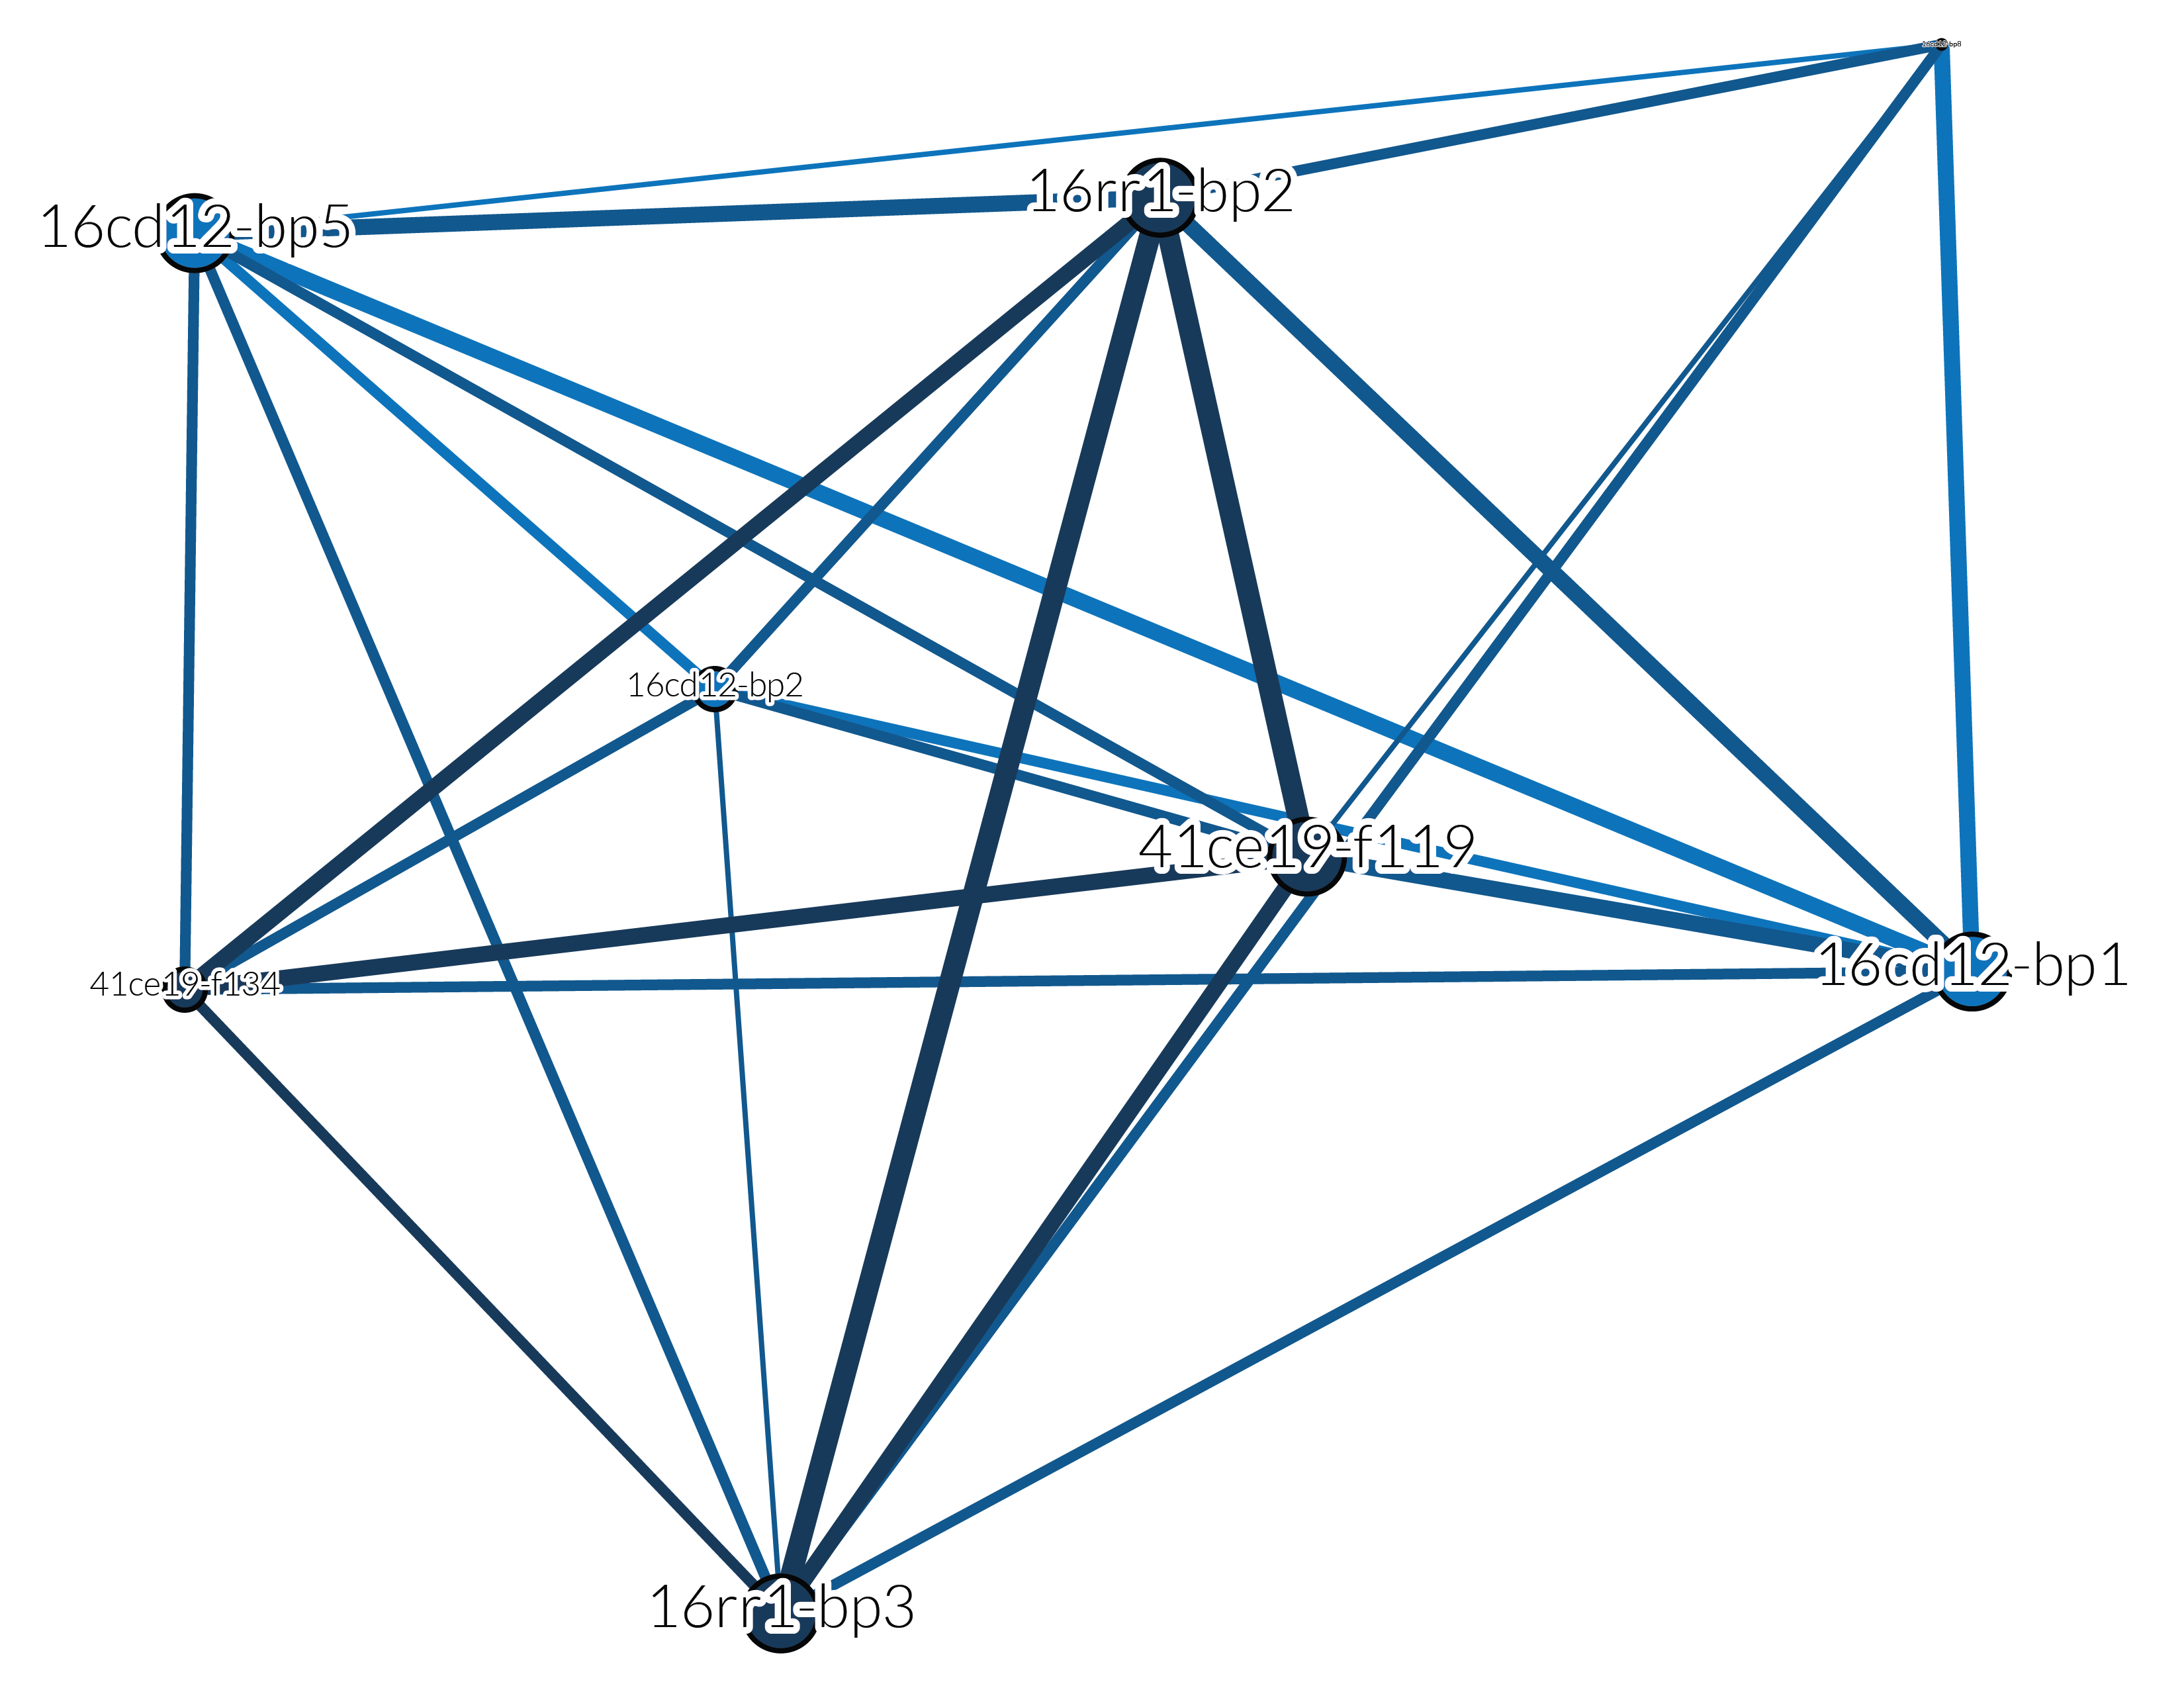
\includegraphics[width=0.8\linewidth]{img/fig04} 

}

\caption{Network of associated diagnostic artifacts recovered with Gahagan bifaces. Nodes are sized by degree, meaning that the larger nodes articulate with a greater number of connections. Node color is defined by the northern (light blue) or southern (dark blue) behavioral regions. Edges are weighted by size and color, meaning that thicker and darker lines represent a greater number diagnostic artifacts that are co-present between contexts.}\label{fig:associated.net}
\end{figure}

\begin{table}
\tbl{Diagnostic artifact types from Caddo burials found in association with Gahagan bifaces.}
{\begin{tabular}{ll} \toprule
Contexts & Diagnostics \\
\midrule
16CD12-BP1 & AL, CA, CC, FR, HA, HE, HFE \\
16CD12-BP2 & AL, HA \\
16CD12-BP5 & AL, FR, HA, SC \\
16CD12-BP8 & CA, HE, HFE, SC \\
16RR1-BP2 & AL, C, HA, HFE, HR, KI, SC \\
16RR1-BP3 & AL, C, HFE, SC \\
41CE19-F119 & AL, C, HA, HFE \\
41CE19-F134 & AL, C, HA \\
\bottomrule
\end{tabular}}
\tabnote{Associated diagnostic artifacts from Caddo burial contexts at the Mounds Plantation (16CD12), Gahagan Mound (16RR1), and George C. Davis (41CE19) sites include Alba arrow points (AL), celts (C), Catahoula arrow points (CA), Coles Creek ceramics (CC), Friley arrow points (FR), Gahagan bifaces (GB), Hayes arrow points (HA), Hickory Engraved ceramics (HE), Holly Fine Engraved ceramics (HFE), Harrell arrow points (HR), Kiam Incised ceramics (KI), and Scallorn arrow points (SC).}
\label{sample-table}
\end{table}

\hypertarget{seriation}{%
\subsection{Seriation}\label{seriation}}

\begin{figure}

{\centering 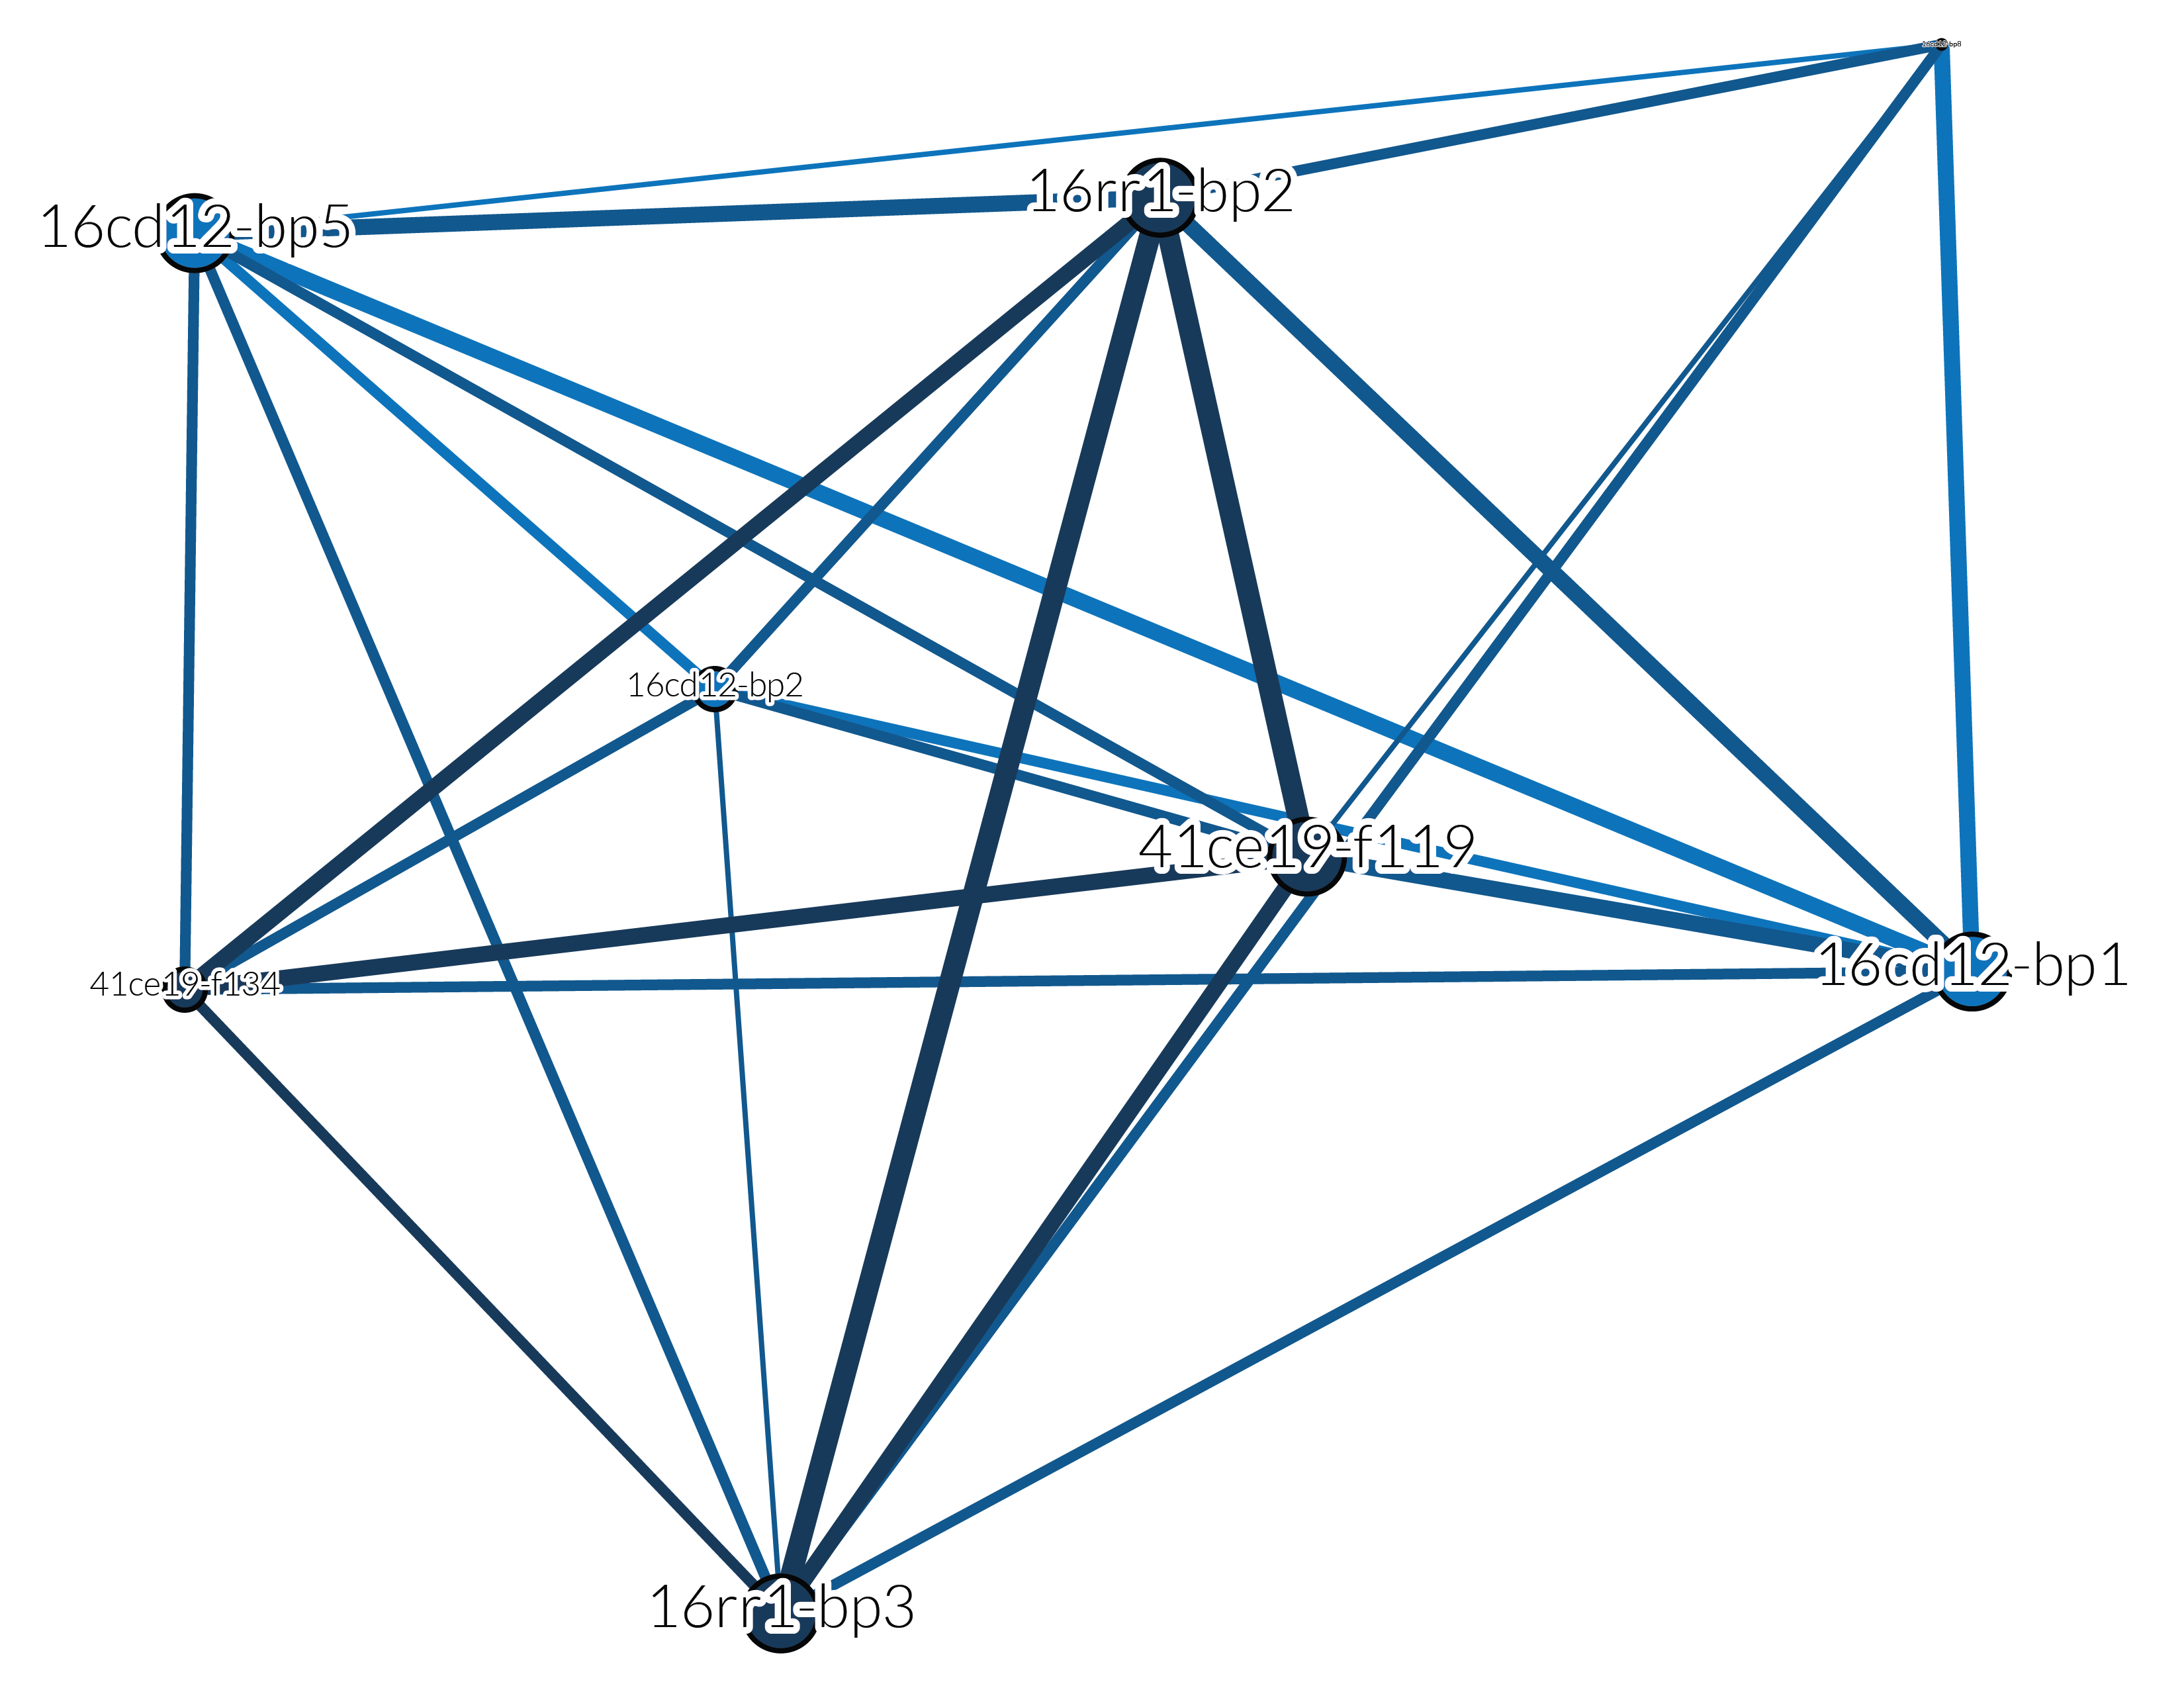
\includegraphics[width=0.8\linewidth]{img/fig03} 

}

\caption{Results of the seriation of Caddo mortuary contexts. Additional information related to the seriation, including those data and code needed to reproduce these results, can be found in the supplemental materials at: https://seldenlab.github.io/gahaganmorph.3/.}\label{fig:h1a}
\end{figure}

\hypertarget{assemblage-diversity}{%
\subsection{Assemblage diversity}\label{assemblage-diversity}}

\hypertarget{d-geometric-morphometrics}{%
\subsection{3D geometric
morphometrics}\label{d-geometric-morphometrics}}

\textbf{Gahagan bifaces included in Caddo burials as a cache differ in
morphology from those placed atop or alongside an individual.}

This hypothesis was tested using Gahagan bifaces from two discrete Caddo
burial practices; one interred as part of a \emph{cache}, and the other
placed atop or alongside \emph{individuals}. Distinct Caddo burial
practices may have been constrained by local morphological requirements,
highlighting aspects of differential design intent.

Data collection procedures are outlined in \cite{RN8154} and
\cite{RN8318}. Characteristic points and tangents used in the
landmarking protocol were inspired by the work of \cite{RN5700}, and the
landmarking protocol is discussed in detail in the
\href{https://seldenlab.github.io/gahaganmorph.3/}{supplementary
materials}.

Landmarks were aligned to a global coordinate system
\citep{RN8102,RN8587,RN8384}, achieved through generalized Procrustes
superimposition \citep{RN8525}, performed in R 4.1.1 \citep{RN8584}
using the \texttt{geomorph} package v4.0.1 \citep{RN8565,RN9565}.
Procrustes superimposition translates, scales, and rotates coordinate
data allowing for comparisons among objects \citep{RN5698,RN8525}. The
\texttt{geomorph} package uses a partial Procrustes superimposition that
projects the aligned specimens into tangent space subsequent to
alignment in preparation for the use of multivariate methods that assume
linear space \citep{RN8511,RN8384}.

Principal components analysis \citep{RN8576,RN10875} was used to
visualize shape variation among the bifaces. The shape changes described
by each principal axis are commonly visualized using thin-plate spline
warping of the landmarks or the reference 3D mesh \citep{RN8555,RN8553}.
A residual randomization permutation procedure (RRPP; n = 10,000
permutations) was used for all Procrustes ANOVAs \citep{RN8579,RN8334},
which has higher statistical power and a greater ability to identify
patterns in the data should they be present \citep{RN6995}. To assess
whether shape differs by context, Procrustes ANOVAs \citep{RN7046} were
run that enlist effect-sizes (z-scores) computed as standard deviates of
the generated sampling distributions \citep{RN8477}. Procrustes variance
was used to discriminate between groups and compare the amount of shape
variation (morphological disparity) across sites \citep{RN5694}, which
is estimated as the Procrustes variance using residuals of linear model
fit \citep{RN8565,RN9565}. A comparison of mean consensus configurations
was used to characterize shape variation in Gahagan bifaces recovered
from contexts where they were found atop or beside an individual or as
part of a cache along the northern wall of the burial pit.

Procrustes ANOVA results indicate a significant difference in Gahagan
biface shape by context (RRPP = 10,000; Rsq = 0.21033;
Pr(\textgreater F) = 1e-04) (Figure 4), and the test for Gahagan biface
(centroid) size by context did not yield a significant result (RRPP =
10,000; Rsq = 0.01138; Pr(\textgreater F) = 0.3933). The test for
morphological disparity by biface size also yielded a significant
result, indicating that the size of bifaces interred atop or alongside
an individual occupy a significantly greater range of morphospace than
those interred as part of a cache.

\begin{figure}

{\centering 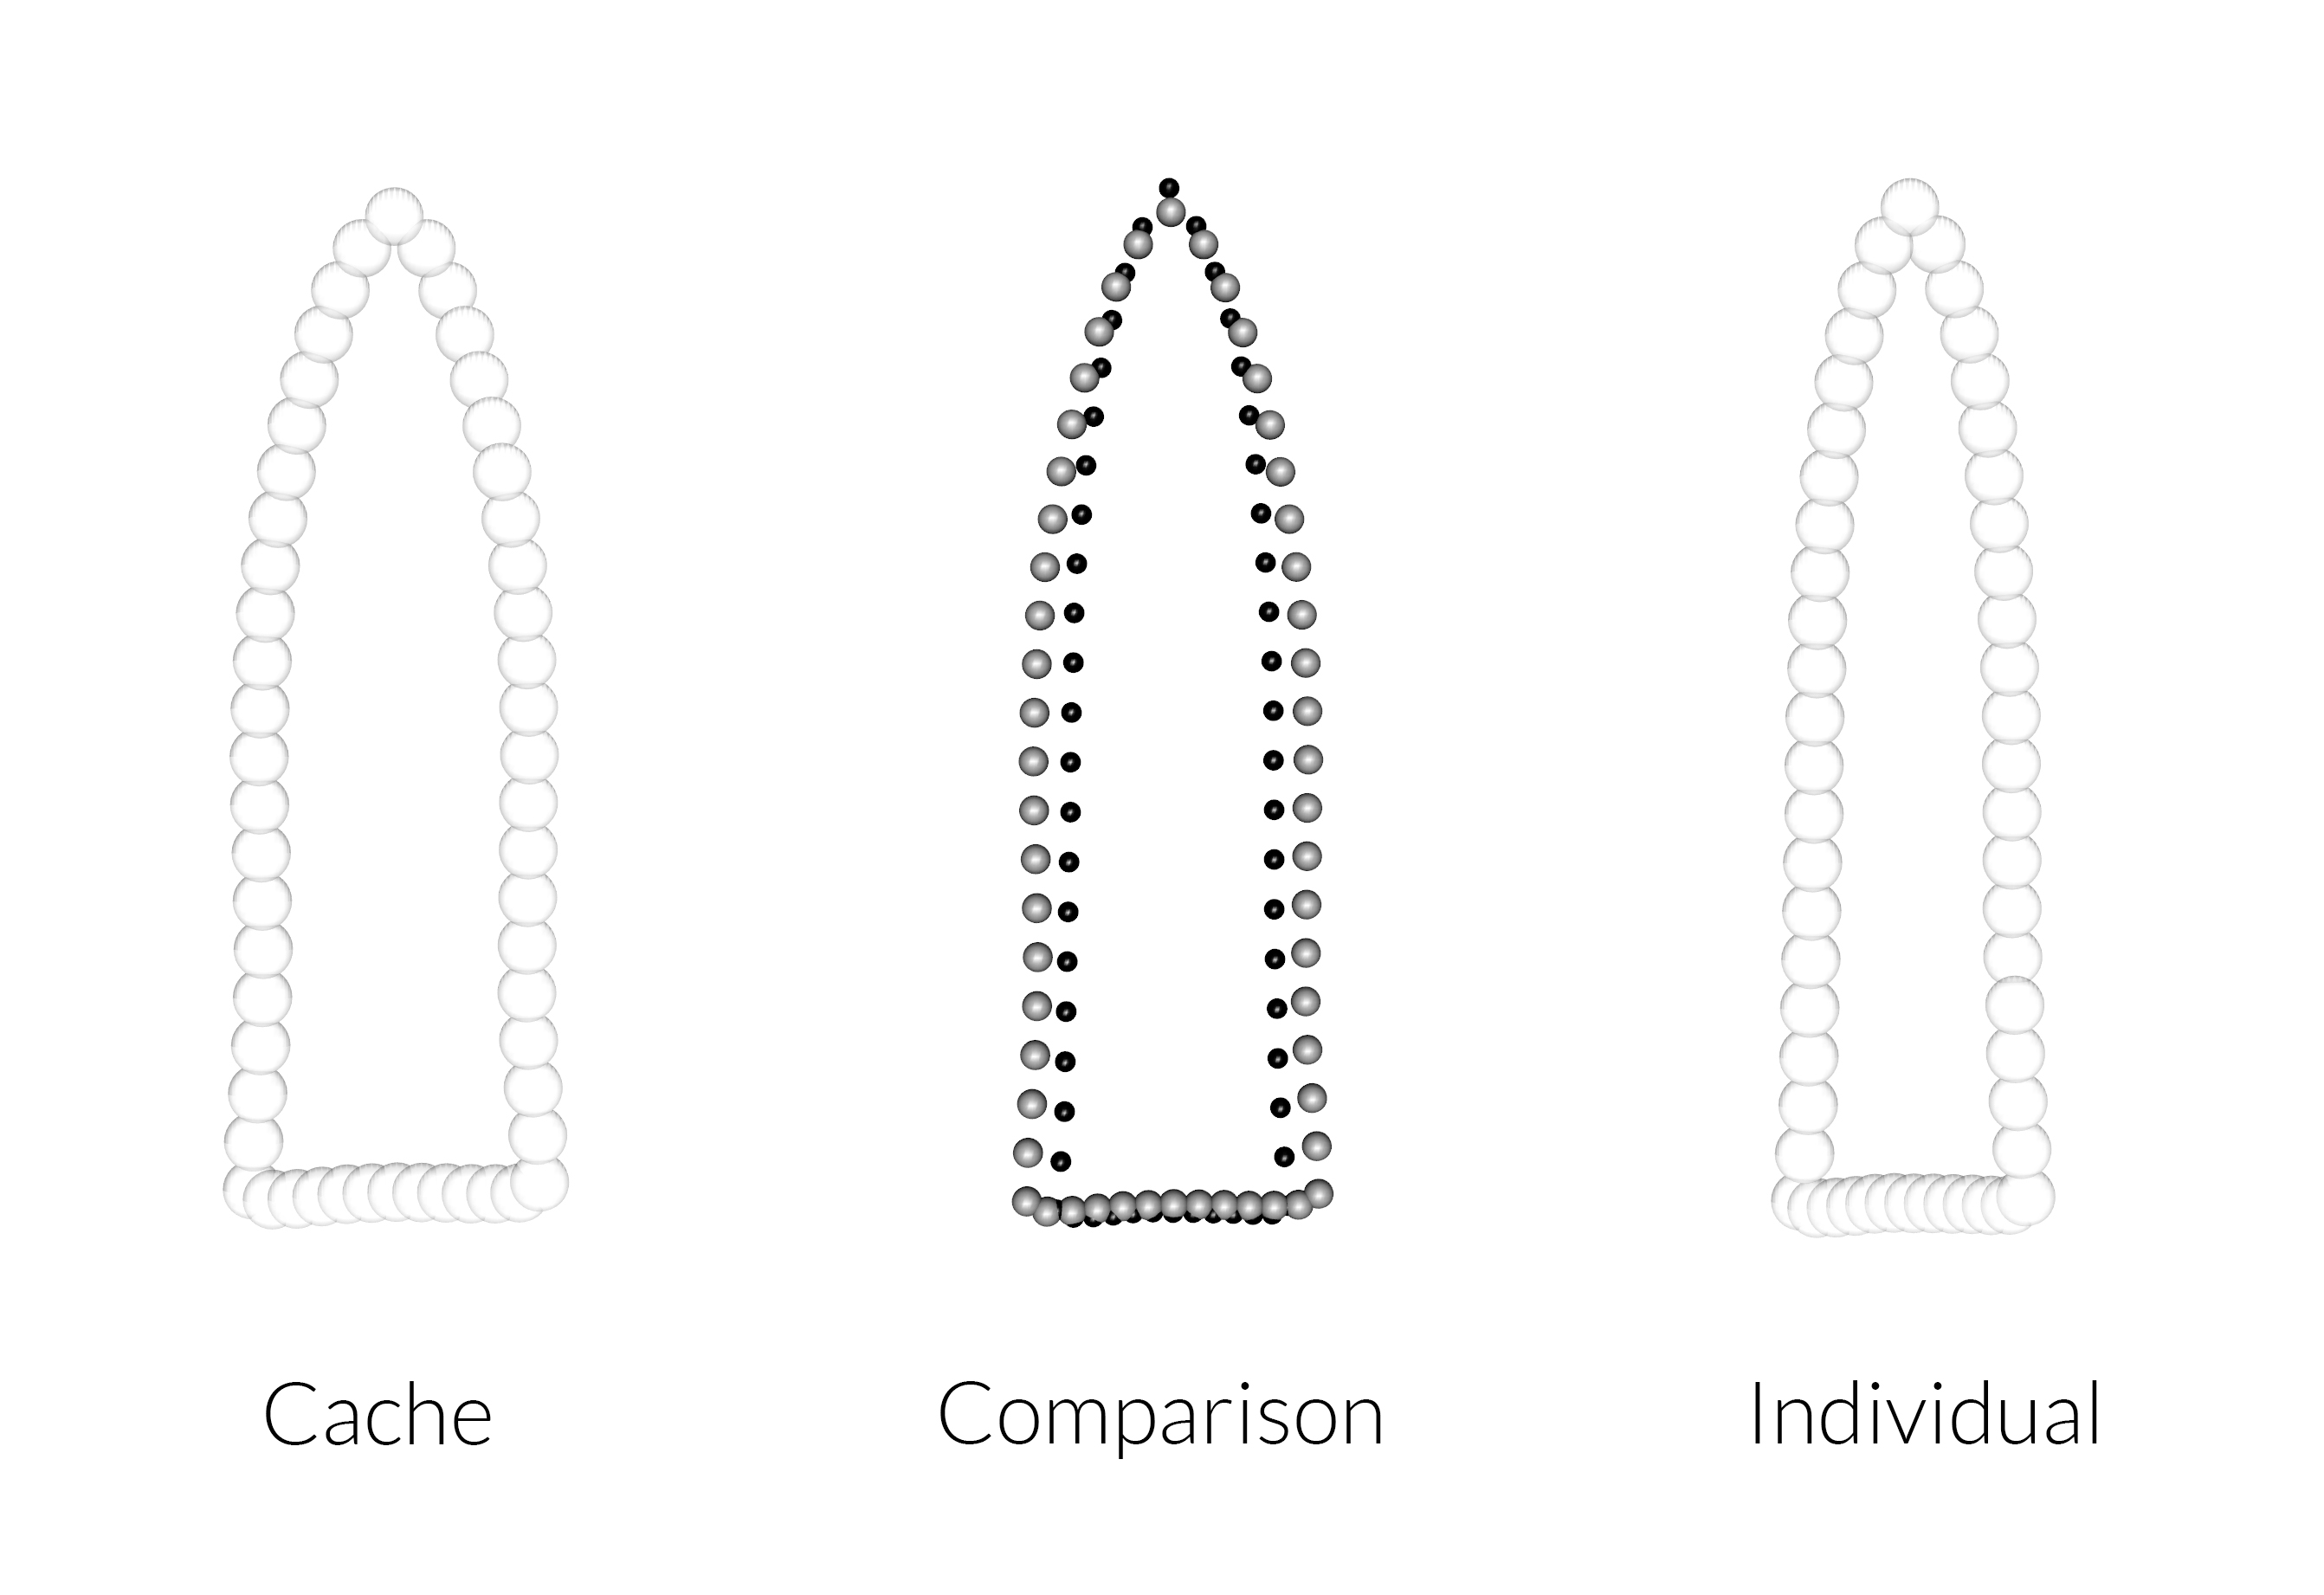
\includegraphics[width=0.9\linewidth]{img/fig05} 

}

\caption{The difference between Gahagan bifaces from cache and individual contexts is characterized by a narrower base, and a reduction in the flexuous blade shape (recurve) for bifaces found atop or alongside Caddo individuals. In the comparison of mean shapes by context, caches are presented in gray, and individuals in black.}\label{fig:mshape.bpractice}
\end{figure}

\hypertarget{discussion}{%
\section{Discussion}\label{discussion}}

Chronometric dates associated with contexts yielding Gahagan bifaces
leave much to be desired, and it is not possible at this time to order
the burial contexts sequentially using the available chronometric data.

\hypertarget{gahagan-biface-morphology-differs-by-burial-context}{%
\subsection{Gahagan biface morphology differs by burial
context}\label{gahagan-biface-morphology-differs-by-burial-context}}

The hypothesis that \emph{Gahagan bifaces included in Caddo burials as a
cache differ in morphology from those placed atop or alongside an
individual} was tested using Gahagan bifaces that articulate with two
distinct Caddo burial practices; one interred as part of a \emph{cache},
and the other placed atop or alongside \emph{individuals}. Burial
practices may have been constrained by local morphological requirements,
highlighting aspects of differential design intent.

Results highlight a significant difference in shape--but not size--for
Gahagan bifaces included with Caddo burials, and significant
morphological disparity in size between the populations. Contextual
differences suggest two Caddo burial traditions associated with Gahagan
bifaces; one more prevalent in the \texttt{northern\ behavioral\ region}
where Gahagan bifaces were placed \emph{atop or alongside an
individual}, and one more prevalent in the
\texttt{southern\ behavioral\ region} where Gahagan bifaces were
\emph{included as a cache offering along the northern periphery of the
burial}. Each burial tradition appears to have been bounded by a
distinct community of practice relating to the placement and shape of
the Gahagan bifaces used in each context.

While the northern community of practice appears to have been in
operation at the same time as that of the southern community of
practice, evidenced by individuals buried at Gahagan Mound and George C.
Davis with Gahagan bifaces placed atop or alongside them, the inverse is
not currently supported by the archaeological record. This raises
questions regarding whether the northern burial tradition predates that
of the south, and/or whether the \texttt{spatial\ boundary} may have
been permeable, but in only one direction.

\hypertarget{conclusion}{%
\section{Conclusion}\label{conclusion}}

\hypertarget{acknowledgments}{%
\section*{Acknowledgments}\label{acknowledgments}}
\addcontentsline{toc}{section}{Acknowledgments}

We extend our gratitude to the Caddo Nation of Oklahoma, the Williamson
Museum at Northwestern State University, the Louisiana State Exhibit
Museum, the Texas Archeological Research Laboratory at The University of
Texas at Austin, the Brazos Valley Museum of Natural History, the Texas
Parks and Wildlife Department, and the Sam Noble Oklahoma Museum of
Natural Science for the requisite permissions and access needed to
generate 3D scans of the Gahagan bifaces. Thanks to Harry J. Shafer,
Hiram F. (Pete) Gregory, Christian S. Hoggard, and David K. Thulman for
their comments on the analyses of Gahagan biface shape.

RZS extends his gratitude to Christian S. Hoggard and David K. Thulman
for their thoughtful comments and constructive criticisms of the
landmarking protocol used in this study
(\href{https://github.com/aksel-blaise/gahaganmorph2/blob/master/analysis/landmarking-protocol.md}{\texttt{LM3d1}}),
as well as the landmarking protocol for Gahagan bifaces that will be
used in the next iteration of these analytical efforts
(\href{https://seldenlab.github.io/gahaganmorph.3/landmarking-protocol-3d2.html}{\texttt{LM3d2}});
to Martin Hinz for fielding questions related to the \texttt{oxcAAR}
package and Derek Hamilton for his guidance with the chronological
models; and to Dean C. Adams, Michael L. Collyer, Emma Sherratt, Lauren
Butaric, and Kersten Bergstrom for their constructive criticisms,
general comments, and suggestions throughout the development of this
research program.

\hypertarget{funding}{%
\section*{Funding}\label{funding}}
\addcontentsline{toc}{section}{Funding}

Components of this analytical work flow were developed and funded by a
Preservation Technology and Training grant (P14AP00138) to RZS from the
National Center for Preservation Technology and Training (NCPTT), and
additional grants to RZS from the Caddo Nation of Oklahoma, National
Forests and Grasslands in Texas (15-PA-11081300-033) and the United
States Forest Service (20-PA-11081300-074). Funding to scan the Gahagan
bifaces at the Williamson Museum at Northwestern State University,
Louisiana State Exhibit Museum, Texas Archeological Research Laboratory
at The University of Texas at Austin, and Sam Noble Oklahoma Museum of
Natural Science was provided to the RZS by the Heritage Research Center
at Stephen F. Austin State University.

\hypertarget{data-management}{%
\section*{Data management}\label{data-management}}
\addcontentsline{toc}{section}{Data management}

The analysis code associated with this project can be accessed through
the supplementary materials
(\url{https://seldenlab.github.io/gahaganmorph.3/}) or the GitHub
repository (\url{https://github.com/seldenlab/gahaganmorph.3}), both of
which are digitally curated on the Open Science Framework
\href{https://osf.io/y7b39/}{DOI: 10.17605/OSF.IO/Y7B39}. The
reproducible nature of this undertaking provides a means for others to
critically assess and evaluate the various analytical components
\citep{RN8312,RN8313,RN8299}, which is a necessary requirement for the
production of reliable knowledge.

Reproducibility projects in \href{https://osf.io/ezcuj/}{psychology} and
\href{https://www.cos.io/rpcb}{cancer biology} are impacting current
research practices across all domains. Examples of reproducible research
are becoming more abundant in archaeology
\citep{RN8207,RN8965,RN8154,RN8318,RN9364,RN11064}, and the next
generation of archaeologists are learning those tools and methods needed
to reproduce and/or replicate research results \citep{RN10760}.
Reproducible and replicable research work flows are often employed at
the highest levels of humanities-based inquiries to mitigate concern or
doubt regarding proper execution, and is of particular import should the
results have---explicitly or implicitly---a major impact on scientific
progress \citep{RN10761}.

\bibliographystyle{tfcad}
\bibliography{biblio.bib}


\input{"appendix.tex"}



\end{document}
